\documentclass[convert={density=300,size=600x600,outfile=\jobname.png}]{standalone}

\usepackage{tikz}
\usetikzlibrary{automata,calc,trees,positioning,arrows,chains,shapes.geometric,%
decorations.pathreplacing,decorations.pathmorphing,shapes,%
matrix,shapes.symbols,plotmarks,decorations.markings,shadows}

\usepackage{subcaption}

\begin{document}

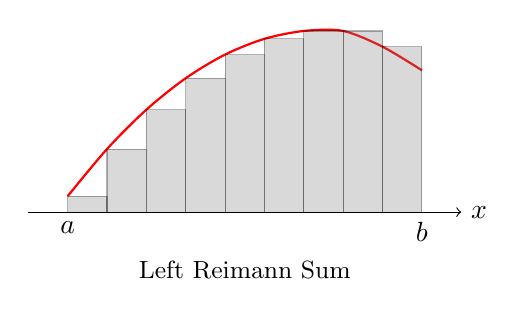
\begin{tikzpicture}[scale=1]
\draw[->] (-0.5,0)--(5,0) node[right] {$x$};
\node[below] at (0,0) {$a$};
\node[below] at (4.5,0) {$b$};
\node[below] at (2.25,-0.5) {\small Left Reimann Sum};
\draw [red, thick] plot [smooth] coordinates { 
	(0.0, 0.20) 
	(0.5, 0.80) 
	(1.0, 1.30)
	(1.5, 1.70)
	(2.0, 2.00)
	(2.5, 2.20)
	(3.0, 2.30)
	(3.5, 2.30)
	(4.0, 2.10)	
	(4.5, 1.80)
};
\draw [black, fill=gray, opacity=0.3] (0.0, 0.00) rectangle (0.5, 0.20);
\draw [black, fill=gray, opacity=0.3] (0.5, 0.00) rectangle (1.0, 0.80);
\draw [black, fill=gray, opacity=0.3] (1.0, 0.00) rectangle (1.5, 1.30);
\draw [black, fill=gray, opacity=0.3] (1.5, 0.00) rectangle (2.0, 1.70);
\draw [black, fill=gray, opacity=0.3] (2.0, 0.00) rectangle (2.5, 2.00);
\draw [black, fill=gray, opacity=0.3] (2.5, 0.00) rectangle (3.0, 2.20);
\draw [black, fill=gray, opacity=0.3] (3.0, 0.00) rectangle (3.5, 2.30);
\draw [black, fill=gray, opacity=0.3] (3.5, 0.00) rectangle (4.0, 2.30);
\draw [black, fill=gray, opacity=0.3] (4.0, 0.00) rectangle (4.5, 2.10);
\end{tikzpicture}
%\caption{Left Riemann Sum}
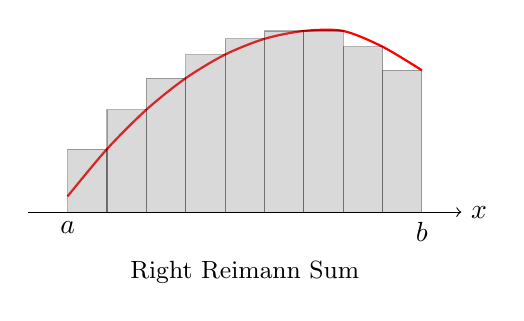
\begin{tikzpicture}[scale=1]
\draw[->] (-0.5,0)--(5,0) node[right] {$x$};
\node[below] at (0,0) {$a$};
\node[below] at (4.5,0) {$b$};
\node[below] at (2.25,-0.5) {\small Right Reimann Sum};
\draw [red, thick] plot [smooth] coordinates { 
	(0.0, 0.20) 
	(0.5, 0.80) 
	(1.0, 1.30)
	(1.5, 1.70)
	(2.0, 2.00)
	(2.5, 2.20)
	(3.0, 2.30)
	(3.5, 2.30)
	(4.0, 2.10)	
	(4.5, 1.80)
};
\draw [black, fill=gray, opacity=0.3] (0.0, 0.00) rectangle (0.5, 0.80);
\draw [black, fill=gray, opacity=0.3] (0.5, 0.00) rectangle (1.0, 1.30);
\draw [black, fill=gray, opacity=0.3] (1.0, 0.00) rectangle (1.5, 1.70);
\draw [black, fill=gray, opacity=0.3] (1.5, 0.00) rectangle (2.0, 2.00);
\draw [black, fill=gray, opacity=0.3] (2.0, 0.00) rectangle (2.5, 2.20);
\draw [black, fill=gray, opacity=0.3] (2.5, 0.00) rectangle (3.0, 2.30);
\draw [black, fill=gray, opacity=0.3] (3.0, 0.00) rectangle (3.5, 2.30);
\draw [black, fill=gray, opacity=0.3] (3.5, 0.00) rectangle (4.0, 2.10);
\draw [black, fill=gray, opacity=0.3] (4.0, 0.00) rectangle (4.5, 1.80);
\end{tikzpicture}
%\caption{Right Riemann Sum}

\end{document}